%   % !TEX root = ../../VIII,3_Rahmen-TeX_8-1.tex
%  
%  
%   Band VIII, 3		Rubrik STOSS
%
%   Signatur/Tex-Datei:	LH_37_05_020
%
%   RK-Nr. 	60278			\ref{RK60278} %??S04
%
%   Überschrift: 	Aequalis processus centri gravitatis
%   
%   Unterrubrik:			DCC plus
%
%   Datierung:		Winter 1676/1677 (?) bis Januar 1678
%
%   edlabels:			0
%
%   Diagramme: 		5
%
%
%   NB: 						(Anmerkungen)					??
%
%
%
\selectlanguage{ngerman}
\frenchspacing
%
\begin{ledgroupsized}[r]{120mm}
\footnotesize
\pstart
\noindent\textbf{Überlieferung:}
\pend
\end{ledgroupsized}
%
\begin{ledgroupsized}[r]{114mm}
\footnotesize
\pstart \parindent -6mm
\makebox[6mm][l]{\textit{L}}%
Aufzeichnung:
LH~XXXVII~5 Bl.~20. 
Ein Blatt~8\textsuperscript{o};
Fragment eines Wasserzeichens in einer Blattecke;
Papiererhaltungsmaßnahmen.
Zwei Seiten.
\pend
\end{ledgroupsized}
%
%
\vspace{5mm}
\begin{ledgroup}
\footnotesize
\pstart
\noindent%
\textbf{Datierungsgründe:}
Ihrem Titel nach ist die vorliegende, skizzenhafte Aufzeichnung N.~\ref{RK60278} %??S04
einem Hauptgegenstand von Leibnizens Untersuchung über die Stoßgesetze gewidmet: der gleichförmigen Bewegung des gemeinsamen Schwerpunkts beim direkten zentralen Stoß zweier Körper.
Im Text N.~\ref{RK60278} %??S04
wird ansatzweise der Fall erörtert, dass die zwei Körper gegenläufig entlang schiefer Ebenen gleiten, die wiederum in einem Fluidum schweben und sich aufeinander bewegen.
Hiermit weist N.~\ref{RK60278} %??S04
inhaltliche Verwandtschaft mit der Aufzeichnung N.~\ref{RK60282} %??S03
auf und knüpft wie diese \textendash\ aber noch deutlicher \textendash\ an Texte an, in denen komplexe Gedankenexperimente das Gesetz der gleichförmigen Bewegung des gemeinsamen Schwerpunkts nachweisen sollten (siehe für die Details die Datierungsbegründung in N.~\ref{RK60282}, %??S03
S.~\pageref{LH_37_05_024_Datierung}).
Auch im Fall von N.~\ref{RK60278} %??S04
aber \textendash\ ebenso wie bei N.~\ref{RK60282} %??S03
\textendash\ fehlt in bemerkenswerter Weise jeder Hinweis darauf, dass das Gesetz über die Bewegung des Schwerpunkts nur dann mit den entworfenen Gedankenexperimenten nachzuweisen sei, wenn zusätzlich die Unmöglichkeit einer \glqq künstlichen immerwährenden Bewegung\grqq\ vorausgesetzt werde.
Demnach treffen auf die Aufzeichnung N.~\ref{RK60278} %??S04
grundsätzlich dieselben Betrachtungen zu, auf denen die Datierung von N.~\ref{RK60282} %??S03
beruht: Der Text könnte zum einen bereits im Winter 1676/1677 verfasst worden sein, während zum anderen
%Auch im Fall von N.~\ref{RK60278} %??S04 
%kommt folglich e
eine Entstehung nach der \textit{Scheda IX de corporum concursu} (N.~\ref{dcc_09}), %??S01\textsubscript{11} 
d.h. nach Januar 1678 nicht in Frage kommt.
Anders aber als bei N.~\ref{RK60282} %??S03
liegt im Träger von N.~\ref{RK60278} %??S04
das Fragment eines Wasserzeichens vor, das im Leibniz-Nachlass nach heutigem Wissensstand lediglich in Handschriften aus den frühen Hannoveraner Jahren anzutreffen ist.
Eine Entstehung der Aufzeichnung N.~\ref{RK60278} %??S04
vor dem Winter 1676/1677 ist folglich in diesem Fall ausgeschlossen.
Hieraus ergibt sich die vorgeschlagene Gesamtdatierung.
%
\pend%
\end{ledgroup}%
%
%
\selectlanguage{latin}%
\frenchspacing%
\count\Bfootins=1000%
\count\Afootins=1200%
\count\Cfootins=1000
\vspace{8mm}%
\pstart%
\normalsize%
\noindent%
%
\lbrack20~r\textsuperscript{o}\rbrack\ %%%% Blatt 20r
\hspace{28mm}
Aequalis processus centri gravitatis\protect\index{Sachverzeichnis}{centrum gravitatis}
\pend%
\vspace{0.5em}%
%\vspace{\baselineskip}
%
\pstart%
\noindent%
Ponantur duae pilae aequales 
%
\edtext{\textit{M}, \textit{N}}{%
\lemma{\textit{M}, \textit{N}}\Cfootnote{%
Die zugehörige fragmentarische Zeichnung ist in \textit{L} gestrichen und wird hier nicht wiedergegeben.}}
%
eadem vi una descendere in \textit{A} in plano inclinato\protect\index{Sachverzeichnis}{planum inclinatum} \textit{AC}, altera 
%
\edtext{descendere in plano inclinato \textit{BD}.
Ipsa autem plana}{%
\lemma{descendere}\Bfootnote{%
\textit{(1)}~altera descendere \textit{B}
\textit{(2)}~in plano inclinato \textit{BD}.
\textit{(a)}~Ipsum autem planum
\textit{(b)}~Ipsa autem plana%
~\textit{L}}} 
%
cogitentur in aequilibrio\protect\index{Sachverzeichnis}{aequilibrium} esse, seu unum descendere alterum ascendere, et ita quidem ut cum \lbrack\textit{Text bricht ab.}\rbrack
\pend%
\pstart%
In planis inclinatis \textit{AB}, \textit{DE},%
\protect\index{Sachverzeichnis}{planum inclinatum}
duo corpora \textit{C}, \textit{F} descendunt.%
\protect\index{Sachverzeichnis}{corpus descendens in plano inclinato}
Ipsa interim plana \makebox[1.0\textwidth][s]{eleventur,
ita ut corpora \textit{C} et \textit{F} sibi occurrant in recta horizonti parallela $C(C)(F)F.$}
\pend
\newpage
% \newpage%
%
%
\centerline{%
\includegraphics[width=0.60\textwidth]{%\hspace{-55mm}
gesamttex/edit_VIII,3/images/LH_37_05_020_d1_020r.pdf%
}} 
\vspace{0.5em}
\centerline{%\hspace{-55mm}
\lbrack\textit{Fig.~1}\rbrack%
}
% \newpage%
\vspace{2.0em}%
%
%
% \vspace*{0.0em} %%%%%%%%% Diagramm 2
\centerline{%
\includegraphics[width=0.50\textwidth]{%\hspace{75mm}
gesamttex/edit_VIII,3/images/LH_37_05_020_d2_020r.pdf%
}}
\vspace{-1.0em}
\centerline{%\hspace{75mm}
\lbrack\textit{Fig.~2}\rbrack%
}
% \newpage%
\vspace{1.5em}
%
\pstart
\noindent
Satius est efficere, ut uno plano descendente alterum ascendat, et uno globo ascendente alter descendat.
%
\lbrack20~v\textsuperscript{o}\rbrack\ %%%% Blatt 20v
%
%\pend%
%%\newpage%
%%
%\pstart%
%\noindent%
In plano 
%
\edtext{autem inclinato%
\protect\index{Sachverzeichnis}{planum inclinatum}%
}{%
\lemma{autem}\Bfootnote{\hspace{-0,5mm}%
\textbar~in \textit{streicht Hrsg.}~%
\textbar\ inclinato%
~\textit{L}}} 
%
necesse est centrum gravitatis%
\protect\index{Sachverzeichnis}{centrum gravitatis}
corporum descendere semper eadem celeritate,
quia in 
%
\edtext{toto ex duobus}{%
\lemma{toto}\Bfootnote{\hspace{-0,5mm}%
\textbar~corpore \textit{gestr.}~%
\textbar\ ex duobus%
~\textit{L}}} 
%
composito eadem est semper gravitas.
\pend%
\pstart%
Duo sint plana%
\protect\index{Sachverzeichnis}{plana parallela}
%
\edtext{parallela et aequalia \textit{CD}, \textit{EF} inclinata%
}{%
\lemma{parallela}\Bfootnote{\hspace{-0,5mm}%
\textbar~\textit{CD} \textit{erg. u. gestr.}~%
\textbar\ et aequalia
\textbar~\textit{CD}, \textit{EF} \textit{erg.}~%
\textbar\ inclinata%
~\textit{L}}}
%
ad horizontem angulo semirecto.%
\protect\index{Sachverzeichnis}{angulus semirectus}
Altitudo unius super horizontem \textit{CF},%
\protect\index{Sachverzeichnis}{horizon}%
\protect\index{Sachverzeichnis}{altitudo}
%
\edtext{nempe \textit{E{\scriptsize \textit{2}}E}, aequalis}{%
\lemma{nempe}\Bfootnote{%
\textit{(1)}~\textit{{\scriptsize 2}CC}, aequalis
\textit{(2)}~\textit{{\scriptsize 1}D{\scriptsize 2}D}, aequalis
\textit{(3)}~\textit{E{\scriptsize \textit{2}}E}, aequalis%
~\textit{L}}}
%
depressioni alterius infra eundem horizontem,%
\protect\index{Sachverzeichnis}{depressio}%
\protect\index{Sachverzeichnis}{horizon}
nempe \textit{D{\scriptsize 2}D}.
Sint \textit{C},
\textit{{\scriptsize 2}D},
\textit{{\scriptsize 2}E},
\textit{F} in eadem recta
et \textit{{\scriptsize 2}D},
\textit{{\scriptsize 2}E} sibi vicina,
ita ut
%
\edtext{duobus existentibus globis%
\protect\index{Sachverzeichnis}{globus}
\textit{A}, \textit{B},
illo descendente in \textit{CD} vi gravitatis,%
\protect\index{Sachverzeichnis}{vis gravitatis}
\lbrack hoc\rbrack\
ascendente in \textit{FE} vi levitatis%
\protect\index{Sachverzeichnis}{vis levitatis}%
\lbrack,\rbrack\
globi%
}{%
\lemma{duobus}\Bfootnote{%\hspace{-0,5mm}%
\textit{(1)}~aequalibus
\textit{(2)}~existentibus
\textit{(a)}~corporibus
\textit{(aa)}~et
\textit{(bb)}~et
\textit{(b)}~globis \textit{A}, \textit{B},
\textbar~illo \textit{erg.}~%
\textbar\ descendente in \textit{CD}
\textit{(aa)}~et
\textbar~hoc \textit{erg.}~%
\textbar\ ascendente
\textit{(bb)}~vi gravitatis,
\textit{(aaa)}~illo in
\textit{(bbb)}~\textbar~illo \textit{ändert Hrsg.}~%
\textbar\ ascendente in \textit{FE} vi levitatis; globi%
~\textit{L}}}
%
concurrant, perinde ac si in recta \textit{CF} concurrissent
(\protect\vphantom)%
semper enim
durante ascensu%
\protect\index{Sachverzeichnis}{ascensus}
et descensu%
\protect\index{Sachverzeichnis}{descensus}
in eadem recta
%
\edtext{manent%
\protect\vphantom(),
in eadem linea directionis semirecta%
\protect\index{Sachverzeichnis}{linea directionis}%
}{%
\lemma{manent\protect\vphantom()}\Bfootnote{%
\textit{(1)}~angulis
\textit{(2)}~linea dir
\textit{(3)}~in eadem linea directionis
\textit{(a)}~ang
\textit{(b)}~semirecta%
~\textit{L}}}
%
ad rectas centra conjungentes.
Patet perinde fore
ac si in rectis immotis
\makebox[1.0\textwidth][s]{\textit{{\scriptsize 2}C{\scriptsize 2}D},
\textit{{\scriptsize 2}F{\scriptsize 2}E}
concurrissent,
adeoque rursus ita descendere.
Ponamus autem rectas \textit{CD},}
\pend
\newpage
%\vspace{0.0em} %%%%%%%%% Diagramm 3
\centerline{%
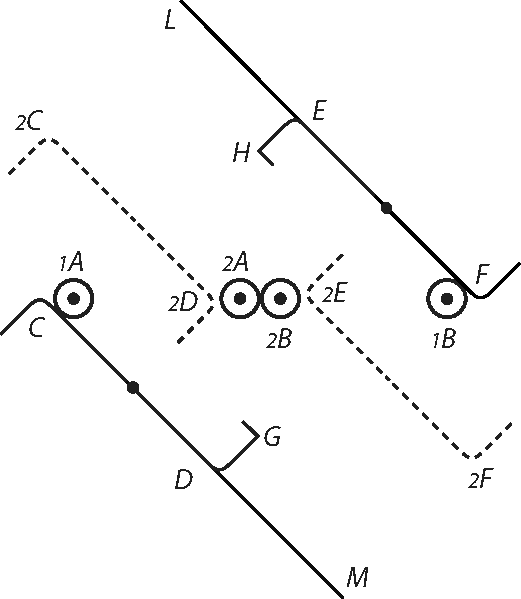
\includegraphics[width=0.50\textwidth]{%
gesamttex/edit_VIII,3/images/LH_37_05_020_d3_020v.pdf%
}}
\vspace{0.5em}
\centerline{%
\lbrack\textit{Fig.~3}\rbrack%
}
\vspace{1.5em}
%%
%%
%%
\pstart
\noindent
\textit{EF} esse in oscillatione%
\protect\index{Sachverzeichnis}{oscillatio}
et\lbrack,\rbrack\
servato parallelismo\lbrack,\rbrack\
contrario motu redire%
\protect\index{Sachverzeichnis}{motus contrarius}
unde venerant,
vel etiam eodem momento
%
\edtext{sibi occurrere}{%
\lemma{sibi}\Bfootnote{%
\textit{(1)}~con
\textit{(2)}~occurrere%
~\textit{L}}}
%
quasi cornibus%
\protect\index{Sachverzeichnis}{cornu}
\textit{EH}, \textit{DG}.
Patet ipsa
ut venerant
descendere\lbrack,\rbrack\
ponendo \textit{LEF}, \textit{MDC} similes et
%
\edlabel{LH_37_05_20v_rkjh-1}%
aequales.%
\edtext{}{%
{\xxref{LH_37_05_20v_rkjh-1}{LH_37_05_20v_rkjh-2}}%
{\lemma{aequales.}\Bfootnote{\hspace{-0,5mm}%
\textit{(1)}~\textlangle Patent non\textrangle\
\textit{(2)}~Aequalia post concursum repercuti, demonstratur
\textbar~communi more \textit{gestr.}~%
\textbar\ ponendo%
~\textit{L}}}}%
%
\pend%
%
\pstart%
Aequalia post concursum repercuti,%
\protect\index{Sachverzeichnis}{repercussio corporum aequalium}%
\protect\index{Sachverzeichnis}{concursus corporum}
demonstratur ponendo%
\edlabel{LH_37_05_20v_rkjh-2}
%
differentiam utcunque parvam.%
\protect\index{Sachverzeichnis}{differentia utcunque parva}
Tunc enim necesse est
ea fere celeritate redire qua venerunt.
Hinc habentur leges concursuum in plano horizontali
%
\edtext{posito dari}{%
\lemma{posito}\Bfootnote{\hspace{-0,5mm}%
\textbar~eas \textit{streicht Hrsg.}~\textbar\ dari%
~\textit{L}}}
%
in casu concurrentium ascendentis et descendentis.
Si angulus,
elevatio%
\protect\index{Sachverzeichnis}{elevatio}
et depressio%
\protect\index{Sachverzeichnis}{depressio}
considerentur ut infinite parva
haberetur jam horizontalis non inclina\textlangle ta.\textrangle
\pend%
\count\Bfootins=1200%
\count\Afootins=1200%
\count\Cfootins=1200
%
%%%% Ende des Textes auf Bl. 20v